\documentclass[11pt]{standalone}
\usepackage{amssymb}
\usepackage{amsmath}
\usepackage[no-math]{fontspec}
\usepackage{unicode-math}
\usepackage{libertinus}
\usepackage{pgf,xcolor}
\usepackage{tikz}
\usetikzlibrary{arrows.meta, backgrounds}
\usepackage{pgfplots}
\pgfplotsset{compat=newest}

\definecolor{my_darkgray}{HTML}{484949}
\definecolor{my_lightgray}{HTML}{F3F4F4}
\definecolor{my_darkblue}{HTML}{005A94}
\definecolor{my_lightblue}{HTML}{CCDEE9}
\definecolor{my_yellow}{HTML}{FFEC7F}
\definecolor{my_red}{HTML}{E60000}
\definecolor{my_orange}{HTML}{E87846}

%% Symmetric rectangular signal (Papula convention):
%%   f(t) = -1 on [-pi, 0),  f(t) = +1 on [0, pi),  T = 2*pi
%%
%% Periodic extension over [-3*pi, 3*pi]:
%%   [-3pi, -2pi): f = -1   (maps to [-pi,  0))
%%   [-2pi,  -pi): f = +1   (maps to [ 0,  pi))
%%   [-pi,    0 ): f = -1
%%   [0,      pi): f = +1
%%   [pi,    2pi): f = -1   (maps to [-pi,  0))
%%   [2pi,   3pi): f = +1   (maps to [ 0,  pi))
%%
%% Numeric values (pi = 3.14159265):
%%   pi  = 3.14159265
%%   2pi = 6.28318530
%%   3pi = 9.42477796

\begin{document}
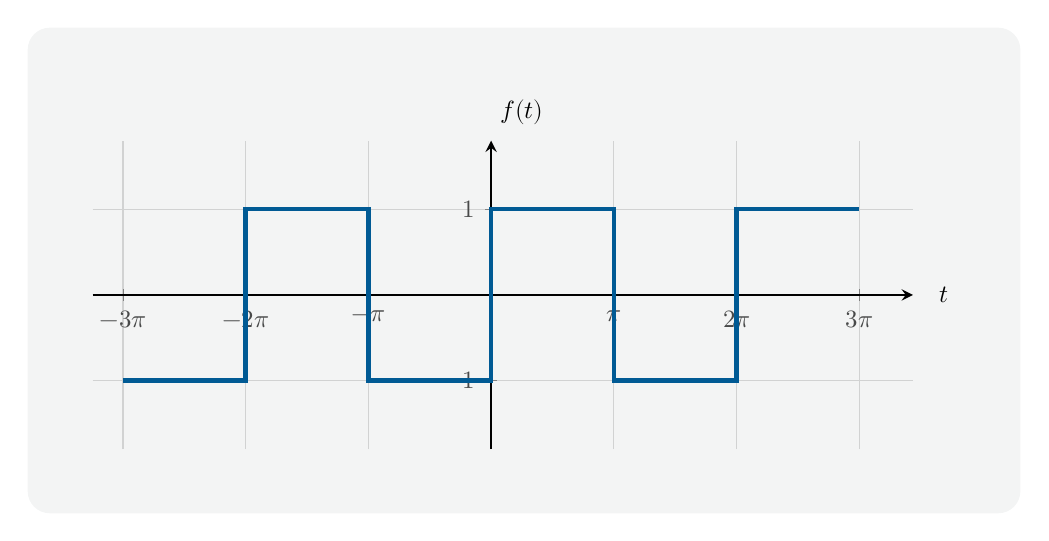
\begin{tikzpicture}[
    show background rectangle,
    background rectangle/.style={fill=my_lightgray, rounded corners=8pt},
    inner frame sep=0.8cm
]

\begin{axis}[
    axis lines = center,
    xlabel = {$t$},
    ylabel = {$f(t)$},
    xlabel style={at={(axis description cs:1.02,0.5)}, anchor=west, font=\small},
    ylabel style={at={(ticklabel* cs:1.02)}, anchor=south west, font=\small},
    xmin = -10.2,
    xmax = 10.8,
    ymin = -1.8,
    ymax = 1.8,
    xtick = {-9.42478, -6.28318, -3.14159, 0, 3.14159, 6.28318, 9.42478},
    xticklabels = {$-3\pi$, $-2\pi$, $-\pi$, $0$, $\pi$, $2\pi$, $3\pi$},
    ytick = {-1, 0, 1},
    yticklabels = {$-1$, $0$, $1$},
    axis line style = {thick},
    grid = both,
    grid style = {draw=my_lightgray!60!white, line width=0.4pt},
    major grid style = {draw=my_lightgray!80!my_darkgray, line width=0.5pt},
    tick label style = {font=\small, color=my_darkgray},
    width = 12cm,
    height = 5.5cm,
    % axis equal not used: y-values are dimensionless +-1, x-values in radians
]

\addplot[
    const plot,
    draw = my_darkblue,
    ultra thick,
    no marks,
]
coordinates {
    (-9.42478, -1)
    (-6.28318,  1)
    (-3.14159, -1)
    ( 0,        1)
    ( 3.14159, -1)
    ( 6.28318,  1)
    ( 9.42478,  1)   %% terminates the last segment at 3*pi
};

\end{axis}

\end{tikzpicture}
\end{document}
